% ===========================
%        Chapter 1A.4
%          Moments
%   Created by Michael Tang
%         2025.02.27
% ===========================

\subsubsection{1A.4 Moments}
\paragraph{Key Definitions}
\begin{itemize}
    \item \textbf{Moment of a force:} The \underline{tendency} (趋势) of a force to cause rotation about a point or
    \underline{pivot} (支点). It is equal to the force multiplied by the perpendicular distance from the pivot to the line of
    action of the force. Formula \footnote{In the formula for moment (or torque):
    \begin{equation*}
        \text{Moment} = F \times d_{\perp}
    \end{equation*}
    the symbol $\perp$ (perpendicular) in $d_{\perp}$ has a specific meaning related to the \underline{lever arm}
    \footnotemark[4] (力臂) in rotational mechanics.
    \begin{itemize}
        \item \textbf{Measuring of $d_{\perp}$:} The quantity $d_{\perp}$ is the  perpendicular distance from the axis of
        rotation (or pivot point) to the line of action of the force $F$. It represents the shortest possible distance between
        the pivot and the force's direction.
        \item \textbf{Use of $d_{\perp}$}
        \begin{itemize}
            \item The movement (torque) measures how effectively a force causes rotation about a pivot.
            \item The greater the perpendicular distance ($d_{\perp}$), the larger the turning effect (moment) for the same
            applied force $F$.
            \item If a force acts directly through the pivot (so $d_{\perp} = 0$), no moment is produced, meaning the force cannot
            create rotation.
        \end{itemize}
    \end{itemize}}:
    \begin{equation}
        \begin{split}
            \text{Moment} &= F \times d_{\perp} \\
            &= Fx
        \end{split}
    \end{equation}
    measured in newton-meters (N$\cdot$m). Sometimes called \underline{torque} (扭矩) or turning force.
    \begin{figure}[H]
        \centering
        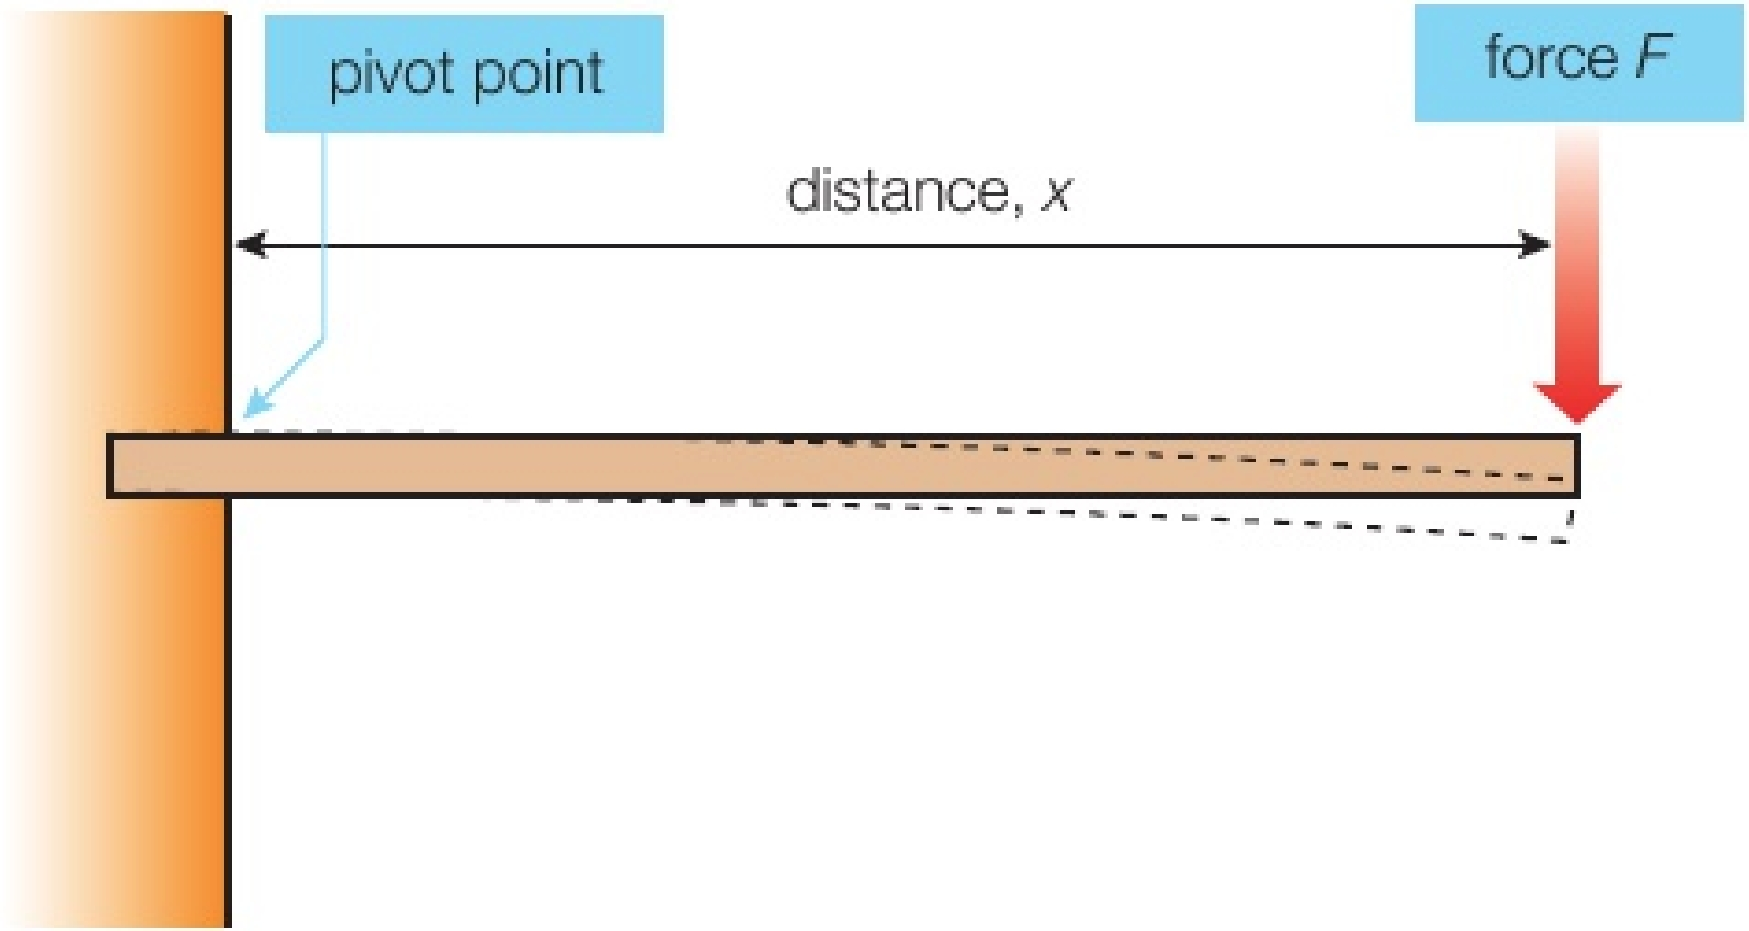
\includegraphics[scale=0.12]{Physics/1A/Images/1A-4-1.png}
        \caption{A force acts on a beam fixed at a point. The movement of a force causes rotation or, in case, blending.}
    \end{figure}
    \begin{figure}[H]
        \centering
        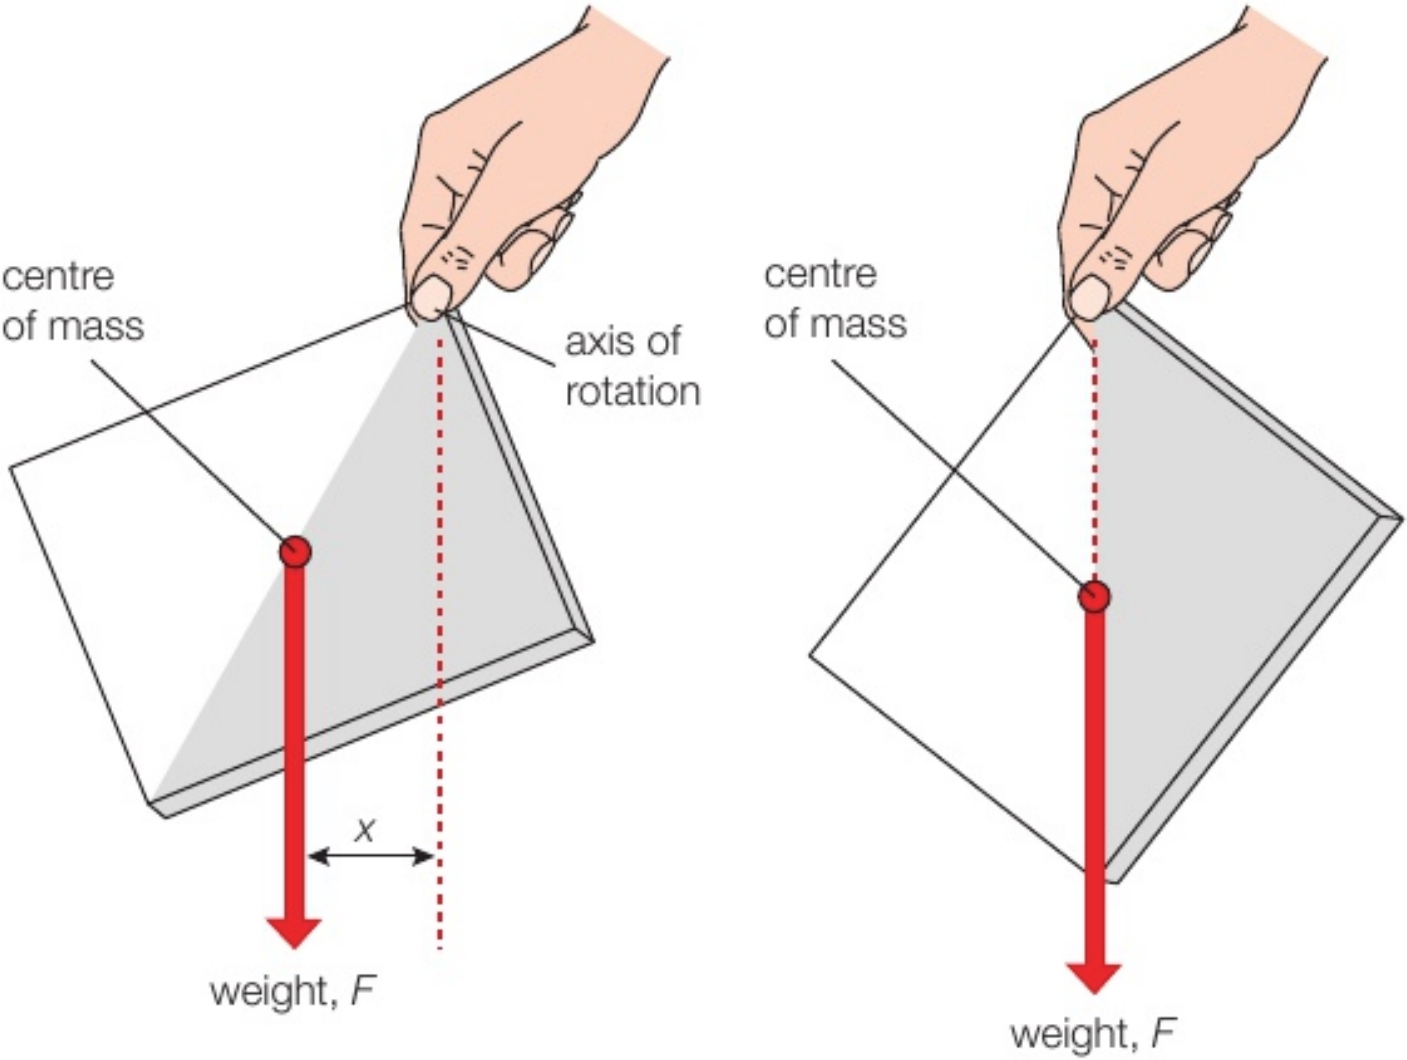
\includegraphics[scale=0.15]{Physics/1A/Images/1A-4-2.png}
        \caption{The calculation of moment only considers the perpendicular distance between the line of action of the force
        and the axis of rotation, through the pivot. When free to retate, a body will turn in the direction of any net moment.}
    \end{figure}
    \item \textbf{Principle of moments:} In equilibrium, for an object that can rotate, the sum of all clockwise moments about
    any pivot equals the sum of all anticlockwise moments about that pivot. This is a condition for rotational equilibrium - no
    \underline{net turning effect} (合力转动效应).
    \item \textbf{Centre of gravity (centre of mass):} The point in an object at which the entire weight can be considered to act.
    In uniform gravity, this \underline{coincides} (符合) with the centre of mass. For \underline{symmetric} (对称) objects, it
    lies at the intersection of symmetry lines. For irregular objects, its position can be found experimentally (e.g., by
    balancing).
    \begin{figure}[H]
        \centering
        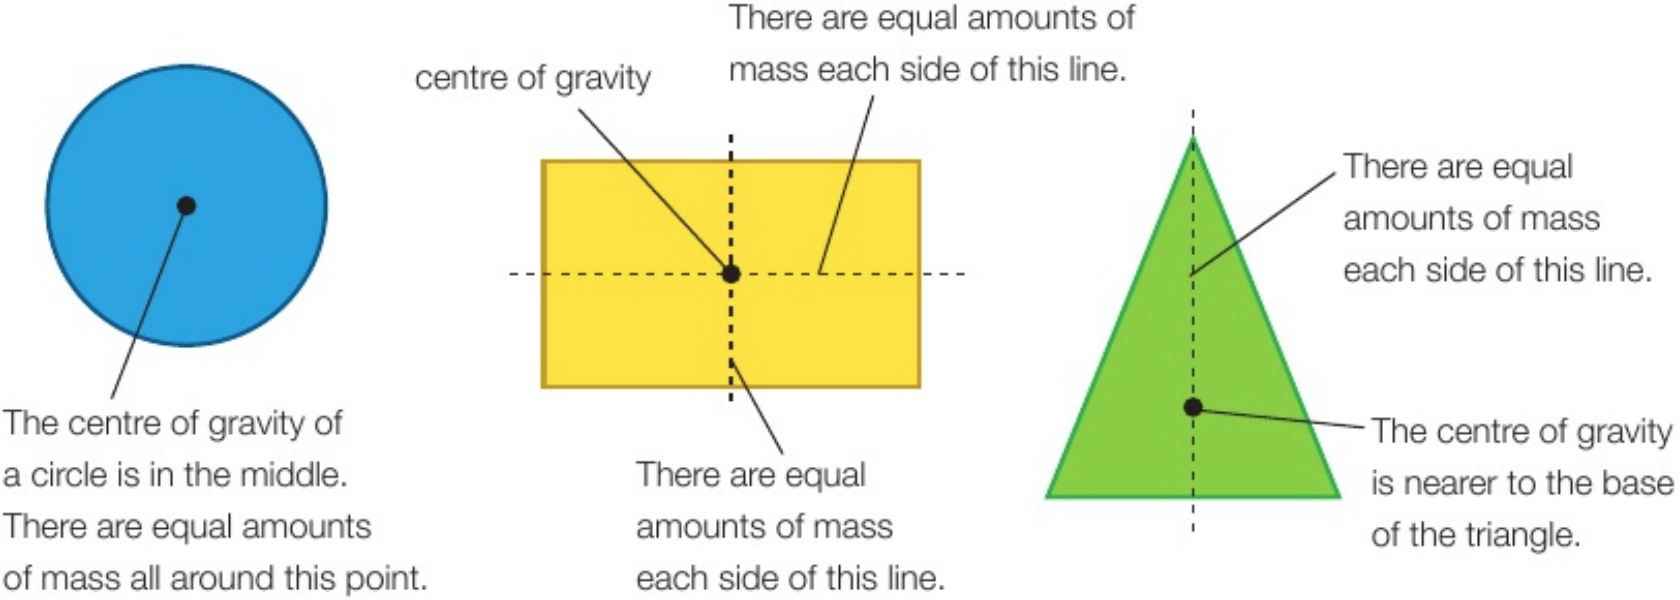
\includegraphics[scale=0.15]{Physics/1A/Images/1A-4-3.png}
        \caption{The centre of gravity of a symmetrical object lies at the intersection of all lines of symmetry.}
    \end{figure}
    \item \textbf{Equilibrium:} A state where a body has zero resultant force and zero resultant moment acting on it, resulting
    in no acceleration (no linear acceleration and no angular acceleration). An object in equilibrium remains at rest or continues
    to move at constant velocity (and, if rotating, at constant angular velocity).
\end{itemize}

\footnotetext[4]{\textbf{Lever arm} is the perpendicular distance from the axis of rotation (pivot point) to the line of action
of the applied force. It determines how effectively the force can cause rotational motion. The lever are is denoted as
$d_{\perp}$, and it can be calculated using:
\begin{equation*}
    d_{\perp} = d \sin{\theta}
\end{equation*}
where $d$ is the distance from the pivot to the point where the force is applied, and $\theta$ is the angle between the force and
the radial line from thee pivot.}

\paragraph{Important Formulae}
\begin{itemize}
    \item \textbf{Moment of a force:}
    \begin{equation}
        \begin{split}
            \text{Moment} &= F \times d_{\perp} \\
            &= Fx
        \end{split}
    \end{equation}
    where $F$ is the force and $d_{\perp}$ is the perpendicular distance from the pivot to the force's line of action.
    \item \textbf{Principle of moments (equilibrium condition):} \footnote{The $\sum$ (sigma) symbol in mathematical notation
    represents summation, which is the process of adding a sequence of numbers. It is commonly used in statistics, calculus, and
    algebra to denote the sum of terms following a specific pattern.
    \begin{itemize}
        \item \textbf{Function of $\sum$}
        \begin{itemize}
            \item It compacts summation expression, replacing long addition sequences with a \underline{concise} (简洁) notation.
            \item It defines a range of summation using lower and upper limits.
            \item It helps in formulating mathematical formulas, especially in series, sequences, and probability.
        \end{itemize}
        \item \textbf{Usage of $\sum$}
        \begin{itemize}
            \item \textbf{General Form}
            \begin{equation*}
                \sum_{i = 1}^{n} f(i) = f(1) + f(2) + f(3) + \cdots + f(n)
            \end{equation*}
            This means adding up all values of $f(i)$ for $i = a$ to $i = b$.
            \item \textbf{Common Applications:}
            \begin{itemize}
                \item Arithmetic and geometric series.
                \item Probability and statistics.
                \item Matrix operations and calculus.
            \end{itemize}
        \end{itemize}
    \end{itemize}}
    \begin{equation}
        \sum M_{\text{clockwise}} = \sum M_{\text{anticlockwise}}
    \end{equation}
    for a system in rotational equilibrium.
    \item \textbf{Centre of gravity via moments:} In a balance \underline{scenario} (情景),
    \begin{equation}
        \begin{split}
            \text{Clockwise Moment} &= \text{Anticlockwise Moment} \\
            mg \times d &= Mg \times x \\
            x &= \frac{md}{M}
        \end{split}
    \end{equation}
    can be used to find the center of gravity of an object of mass $M$ balanced by a smaller mass $m$ at a known distance $d$
    ($g$ cancels out), while $x$ is the distance from the pivot to the center of gravity.
\end{itemize}

\paragraph{Theoretical Concepts}
\textbf{Moment (Turning Effect) of a Force}
A force can only push or pull an object in a line, but also make it turn or rotate about a pivot. The moment (or turning effect)
of a force quantifies how much the force tends to rotate the object. It depends on two factors:
\begin{itemize}
    \item The magnitude of the force $F$.
    \item The perpendicular distance $d_{\perp}$ from the pivot to the line of action of the force.
\end{itemize}
A larger force or a longer \underline{leverage} (杠杆作用, distance) gives a larger moment. \par
For example, pushing a door near the \underline{hinges} (铰链) \underline{versus} (相对于) at the handle: the same force at the
handle (far from the hinges) produces a greater moment (easier to rotate the door) than near the hinge. The direction of rotation
can be specified as clockwise or anticlockwise based on the force's tendency. \par
\textbf{Why perpendicular distance?} Only the component of the force that is perpendicular to the line from the pivot causes
rotation. If a force acts directly through the pivot ($d_{\perp} = 0$), it produces no moment (no rotation). If the force is at
an angle, we always take the perpendicular distance to calculate the effective turning leverage. \underline{Equivalently} (等效于),
one can use the component of the force perpendicular to the lever arm.

\paragraph{Equilibrium and the Principle of Moments}
For an object to be in equilibrium (completely balanced and not accelerating in any way), two conditions must me met:
\begin{itemize}
    \item[1.] The resultant force on it is zero (no linear acceleration).
    \item[2.] The resultant moment on it is zero (no angular acceleration).
\end{itemize} \par
The second condition is the principle of moments in action: all the clockwise moments about any chosen pivot must equal all the
anticlockwise moments. When this holds, the net turning effect is zero, so the object will not start to rotate (or if already
rotating, it continues at constant angular speed). \par
In practical terms, to apply the principle of moments:
\begin{itemize}
    \item Choose a pivot point (often a support or hinge).
    \item Calculate the moment of each force about that pivot. Take care to assign a sense to each moment.
    \item Set the sum of clockwise moments equal to the sum of anticlockwise moments if the object is balanced.
    \item Solve for the unknown if required.
\end{itemize} \par
This principle is used in many contexts, e.g. balancing \underline{beams} (梁), seesaws, weighing scales, and determining forces
on supports. Each individual moment was calculated, then summed for clockwise and equated to the sum of anticlockwise moments to
solve for the unknown weight of the beam.

\paragraph{Solving Moment Problems - Strategy}
In moment problems, list all forces and their distances from the chosen pivot. Decide which side (or direction of rotation) each
force would cause. Then write an equation equating the total moment causing clockwise rotation to the total moment causing
anticlockwise rotation (if in equilibrium). If not in equilibrium, we might be computing a net moment instead. \par
\textbf{Important:} We cannot add forces directly to get a total moment; we must add their moments. \par
Also, ensure consistent units (convert all distances to meters, forces to newtons). The solution should be laid out with clear
steps: identify pivot, write down moments on each side, etc., to get high marks. This approach also reduces mistakes.

\paragraph{Center of Gravity (Center of Mass)}
The center of gravity of an object is the point at which the weight of the object can be considered to act. In
\underline{uniform gravity} \footnote{\textbf{Uniform garvity:} In physics, uniform gravity refers to a \underline{gravitational
field} \footnotemark[6] (引力场) in which the acceleration due to gravity is constant in both magnitude and direction throughout a
given region. This assumption simplifies calculations and is commonly used in problems involving motion near the Earth's surface,
where gravitational acceleration ($g$) is approximately $9.81 \unit{m.s^{-2}}$ and acts downward.} (均衡重力场), it's the same as
the object's center of mass. If support an object at its center of gravity, it will balance perfectly (no net moment due to
gravity on either side). For regularly shaped, uniform objects, the center of gravity is at the geometric center or along lines
of symmetry. \par

\footnotetext[6]{\textbf{Gravitational field:} A gravitational field is a region in space where a mass experiences a gravitational
force due to the presence of another mass. The strength and direction of the field at any point are defined by the gravitational
field strength ($g$), which is the force per unit mass \underline{exerted} (施加) on a small test mass placed at that point. \par
\textbf{Center of gravity vs. center of mass:} For most physics problems on Earth, we treat them as the same point. A Learning
Tip in the textbook notes that the terms can be used interchangeably for objects that are small relative to Earth. Only in varying
gravitational fields would the \underline{distinction} (区别) matter.

Mathematically, it is expressed as:
\begin{equation*}
    g = \frac{F}{m}
\end{equation*}
where $F$ is the gravitational force experienced by an object of mass $m$. \par
\textbf{Types of Gravitational Fields}
\begin{itemize}
    \item \textbf{\underline{Uniform Gravitational Field} (均匀重力场)}
    \begin{itemize}
        \item In small regions, such as near Earth's surface, gravity can be approximated as \underline{uniform} (均一的).
        \item The field lines are parallel and equally spaced, indicating that the gravitational force is the same in magnitude
        and direction at every point.
        \item The acceleration due to gravity is nearly constant at $9.81 \text{m/s}^2$ near Earth's surface.
    \end{itemize}
    \item \textbf{\underline{Radial Gravitational Field} (径向重力场)}
    \begin{itemize}
        \item For larger distances from a mass (such as planets or stars), the gravitational field is no longer uniform but
        radial.
        \item The strength of the field follows Newton's \underline{inverse-square law} \footnotemark[7] (平方反比定律), given by:
        \begin{equation*}
            g = \frac{GM}{r^2}
        \end{equation*}
        where:
        \begin{itemize}
            \item $g$ is the gravitational field strength.
            \item $G$ is the gravitational constant ($6.67 \times 10^{-11} \unit{N.m^2.kg^{-2}}$).
            \item $M$ is the mass creating the gravitational field.
            \item $r$ is the distance from the center of the mass of the object.
            \item The field lines point radially inward, indicating that gravity always pulls objects toward the center of the
            mass causing the field.
        \end{itemize}
    \end{itemize}
\end{itemize} \par
\textbf{Key Properties of a Gravitational Field}
\begin{itemize}
    \item \textbf{Attractive Force:} Gravity always pulls masses toward each other; it never repels.
    \item \textbf{Infinite Range:} Although gravity weakens with distance, it theoretically extends to infinity.
    \item \textbf{Superposition Principle:} The resultant gravitational field at any point due to multiple masses is the vector
    sum of the individual fields.
\end{itemize} \par
In \underline{astrophysics} (天体物理学), gravitational fields determine planetary \underline{orbits} (轨道), \underline{tides}
(潮汐), and even the bending of light in strong gravitational fields (\underline{gravitational lensing} (引力透镜效应)).}

\footnotetext[7]{\textbf{Inverse-Square Law:} The inverse-square law states that a physical quantity (such as gravitational force,
electric field, or light intensity) decreases in proportion to the square of the distance from the source. This principle applies
to gravity, where the gravitational field strength ($g$) and gravitational force ($F$) follow the relationship:
\begin{equation*}
    F = \frac{GMm}{r^2}
\end{equation*}
where:
\begin{itemize}
    \item $F$ is the gravitational force between two masses.
    \item $G$ is the gravitational constant ($6.67 \times 10^{-11} \unit{N.m^2.kg^{-2}}$).
    \item $M$ and $m$ are the masses involved.
    \item $r$ is the distance between their centers of mass.
\end{itemize} \par
\textbf{Gravitational Field Strength and Inverse-Square Law} \par
The gravitational field strength ($g$) at a distance $r$ from a mass $M$ is given by:
\begin{equation*}
    g = \frac{F}{m} = \frac{GM}{r^2}
\end{equation*} \par
This equation shows that as the distance $r$ doubles, the gravitational field strength becomes one-forth of its original value:
\begin{equation*}
    g' = \frac{GM}{\left(2r\right)^2} = \frac{GM}{4r^2} = \frac{1}{4} g
\end{equation*} \par
\textbf{General Mathematical Form of the Inverse-Square Law} \par
For any physical quantity $I$ (such as intensity of light, force, or field strength) that follows the inverse-square law:
\begin{equation*}
    I \propto \frac{1}{r^2}
\end{equation*}
which can be written as:
\begin{equation*}
    I = \frac{k}{r^2}
\end{equation*}
where $k$ is a constant depending on the system. This relation holds for:
\begin{itemize}
    \item \textbf{Gravitational Force}
    \begin{equation*}
        F = \frac{GMm}{r^2}
    \end{equation*}
    \item \textbf{Gravitational Field Strength}
    \begin{equation*}
        g = \frac{GM}{r^2}
    \end{equation*}
    \item \textbf{Electric Field Strength (Coulomb's Law)}
    \begin{equation*}
        E = \frac{kQ}{r^2}
    \end{equation*}
    \item \textbf{Intensity of Light}
    \begin{equation*}
        I = \frac{k}{r^2}
    \end{equation*}
\end{itemize} \par
\textbf{Visualization of the Inverse-Square Law} \par
A simple way to understand the inverse-square law is to visualize how the influence of a source spreads over an increasing area.
\par
\textbf{Area Expression Concept:} The surface area of a sphere increases with the square of the radius:
\begin{equation*}
    A = 4 \pi r^2
\end{equation*}
Since the same amount of force or energy is spread over this area, the intensity at a given point decreases proportionally:
\begin{equation*}
    I = \frac{\text{Total Energy or Force}}{4 \pi r^2}
\end{equation*} \par
\textbf{Diagram Representation}
\begin{center}
    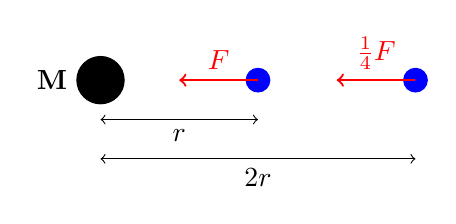
\begin{tikzpicture}
    % Central mass M
    \filldraw[black] (0,0) circle (0.3) node[left=0.3cm] {\textbf{M}};
    
    % Two test masses at distances r and 2r
    \filldraw[blue] (2,0) circle (0.15);
    \filldraw[blue] (4,0) circle (0.15);
    
    % Arrows representing force
    \draw[->, red, thick] (2,0) -- (1,0) node[midway, above] {$F$};
    \draw[->, red, thick] (4,0) -- (3,0) node[midway, above] {$\frac{1}{4}F$};
    
    % Distance labels
    \draw[<->] (0,-0.5) -- (2,-0.5) node[midway, below] {$r$};
    \draw[<->] (0,-1) -- (4,-1) node[midway, below] {$2r$};
    \end{tikzpicture}
\end{center}
where:
\begin{itemize}
    \item Mass $M$ at the center of generates a gravitational field.
    \item Test mass at distance $r$ experiences a force $F$.
    \item Test mass at distance $2r$ experiences a force $\frac{1}{4}F$.
    \item The arrows represent gravitational force decreasing as distance increases.
\end{itemize}}

For irregular objects or non-uniform objects, the center of gravity is not obvious by symmetry. We can find it experimentally by
the principle of moments or by suspension: e.g., we can balance the object on a narrow support (like finding the balance point of
a broom). In the broom experiment, a known smaller mass was used to balance the broom at a certain point; by equating moments
(mass $\times$ distance), the distance to the broom's center of gravity could be calculated. Another simple method is to hang the
object from different points and use a plumb line - the lines of action of gravity will intersect at the center of gravity.